\documentclass[10pt, letterpaper]{scrartcl}
\usepackage[top=2.5cm, bottom=2.5cm, left=2.5cm, right=2.5cm]{geometry}
\usepackage[utf8]{inputenc}
\usepackage{amsmath}
\usepackage{amsfonts}
\usepackage{amssymb}
\usepackage{xspace}
% double spacing recommended by Microwave Magazine for review process
\usepackage{setspace}
\doublespacing

\usepackage{color,array}

\usepackage{graphicx}
\usepackage{siunitx}
\usepackage[labelformat=simple]{subfig}
\renewcommand{\thesubfigure}{(\alph{subfigure})}    % creates parentheses for "Fig. 1(a)"

\usepackage{hyperref}
\hypersetup{
	colorlinks=true,
	linkcolor=blue,
	filecolor=magenta,      
	urlcolor=cyan,
	citecolor=blue
}

%% Python listing def
\usepackage{listings}
\definecolor{codegreen}{rgb}{0,0.6,0}
\definecolor{codegray}{rgb}{0.5,0.5,0.5}
\definecolor{codepurple}{rgb}{0.58,0,0.82}
\definecolor{backcolour}{rgb}{0.95,0.95,0.92}
\lstdefinestyle{mystyle}{
	backgroundcolor=\color{backcolour},  
	commentstyle=\color{codegreen},
	keywordstyle=\color{magenta},
	numberstyle=\tiny\color{codegray},
	stringstyle=\color{codepurple},
	basicstyle=\footnotesize,
	breakatwhitespace=false,        
	breaklines=true,                
	captionpos=b,                   
	keepspaces=true,                
	numbers=left,                   
	numbersep=5pt,                 
	showspaces=false,               
	showstringspaces=false,
	showtabs=false,                 
	tabsize=2
}
\lstset{style=mystyle}

% alias for scikit-rf (without capitalization)
\newcommand{\skrf}{{s}cikit-rf\xspace}

\title{\skrf{}: An Open Source Python Package for Microwave Network Creation, Analysis and Calibration} 

% After Alex, should we  proceed by GitHub contributor ranking or by alphabetical order ?
% GitHub list of contributors
% https://github.com/scikit-rf/scikit-rf/graphs/contributors
%
\author{Alexander Arsenovic, % 810 Labs LLC
	    Julien Hillairet, % CEA, IRFM, F-13108 St-Paul-Lez-Durance, France (julien.hillairet@cea.fr)
		Jackson Anderson, % Purdue University, West Lafayette, Indiana, USA (ander906@purdue.edu)
		Henrik Forsten, \\ % MilliLab, VTT Technical Research Center of Finland, 02044 Espoo, Finland (henrik.forsten@vtt.fi)
		Vincent Rieß, % AES GmbH, Hanna-Kunath-Str. 33 28199 Bremen, Germany (vincent.riess@aes-aero.com)
 		Michael Eller, % University of Virginia, Virginia, USA (mbe9a@virginia.edu)
		Noah Sauber, % University of Virginia, Virginia, USA (nds5yf@virginia.edu)
		Robert Weikle, \\ % University of Virginia, Virginia, USA (rmw5w@virginia.edu)
		William Barnhart, % HawkEye 360, 196 Van Buren Street, Suite 450, Herndon, VA 20170 (william.barnhart@he360.com)
		Franz Forstmayr, % Rosenberger Hochfrequenztechnik GmbH & Co. KG, Hauptstraße 1, 83413 Fridolfing, Germany (franz.forstmayr@rosenberger.com)
		and GitHub Contributors\footnote{\url{https://github.com/scikit-rf/scikit-rf/graphs/contributors}},  %https://github.com/scikit-rf/scikit-rf/graphs/contributors
	}

%CORRESPONDING AUTHOR: A. Arsenovic (e-mail: \href{mailto:alex@810lab.com}{alex@810lab.com}).

\date{}

% an abstract is not required/allowed for the Mircowave Magazine
%\begin{abstract}
%Measurements at microwave frequencies can require a  significant  amount of post-processing  and  analysis,  especially  in research  and  prototyping environments.  From  our  experience, none  of   the   existing   software   products  satisfy   the   needs   of these environments in which the abilities to understand, modify, and  extend  existing  functionality  are  vital.  In  an  attempt  to provide this  needed  functionality,  we  have  created  \skrf{};  an open  source,  BSD-licensed  package  for  microwave  engineering implemented   in   the   Python  programming   language.   \skrf{} seeks  to  provide  a  modern,  object-oriented  library  for  network analysis  and  calibration  aimed  at  being  flexible  and scalable. In  this  paper,  we  introduce  the  motivation  behind  the  \skrf{}  project   and   demonstrate  its  current   abilities   with   some example applications.
%\end{abstract}

%\begin{IEEEkeywords}
%Scientific computing, Object oriented programming, Network theory, Circuit analysis, Circuit simulation, Microwave circuits
%\end{IEEEkeywords}



\begin{document}


% make the title area
\maketitle

\section{Context and Motivations}
With the rapid proliferation of telecommunication and radio-frequency (RF) applications, so too has demand grown for tools to design and characterize these devices. \skrf{} is a Python package designed to make RF/Microwave engineering both robust and approachable. The package provides a modern, object-oriented library for RF network analysis, circuit building, calibration, and simulation. Besides offering standard microwave network operations, such as reading/writing Touchstone files (\texttt{.sNp} files), connecting or de-embedding $N$-port networks, frequency/port slicing, concatenation or interpolations, it is also capable of advanced operations such as Vector Network Analyzer (VNA) calibrations, time-gating, vector fitting, interpolating between an individual set of networks, deriving network statistical properties and support of Virtual Instruments for direct communication to VNAs. The package also allows straightforward plotting of rectangular plots (dB, magnitude, phase, group delay, etc.), Smith Charts or automated uncertainty bounds.
 
The project was created in 2009 and has been continually developed since. The package is distributed under the Berkeley Software Distribution (BSD) licence and is actively developed by more than 50 volunteers on GitHub. The project has users in several universities and research institutes around the world as well as corporate users from large companies including Keysight, Rohde \& Schwarz, National Instruments, Nvidia, and 3M. As of 2021, the package has been downloaded more than 220,000 times since its creation and has been used in over thirty publications.

As the package is developed in Python, it makes it naturally compatible with the rich set of modern scientific Python libraries. Results can be shared and directly reproduced by other researchers using tools such as Binder or Google Colab. Being a Python library, it is also compatible with the robust testing and code coverage frameworks developed for the language, with reproducible modelling approaches using online virtualization services. Being open-source, users of \skrf{} are able to see exactly what the source code is doing and, if a feature does not exist, are able to freely contribute it to extend the library for their work and for others. And, of course, it is free.

\section{Basic Usage of \skrf{}}

Detailed installation instructions can be found in the \skrf{} documentation (\url{https://scikit-rf.readthedocs.io/en/latest/}). For those familiar with Python, it is no different from installing any other package, being distributed through both pip and Conda. After installation, the package can be imported, which is assumed for all the following examples:
\begin{lstlisting}[language=Python]
import skrf
\end{lstlisting}

The following sections outline some fundamental features of \skrf{}, and include code snippets to provide a starting point for new users.

\subsection{Reading and Plotting Networks}

The central object in the \skrf{} package is a $N$-port microwave \texttt{Network} object. A \texttt{Network} can be created in various ways, for example by reading a Touchstone file named \texttt{measured\_data.s2p}:

\begin{lstlisting}[language=Python]
example_network = skrf.Network('measured_data.s2p')
\end{lstlisting}

In order for the reader to reproduce the given examples, a test-case is provided in the package and can be imported via:

\begin{lstlisting}[language=Python]
>>> from skrf.data import ring_slot
>>> ring_slot
2-Port Network: 'ring slot',  75.0-110.0 GHz, 201 pts, z0=[50.+0.j 50.+0.j]
\end{lstlisting}

The basic attributes of a microwave network are provided by the following properties of the \texttt{Network} class:
\begin{itemize}
\item \texttt{s}: Scattering parameter matrix.
\item \texttt{z0}: Port impedance matrix.
\item \texttt{frequency}: Frequency object.
\end{itemize}

S-parameters are represented by a ($n_{bf} \times N \times N$) NumPy array \cite{harris2020} (\url{https://numpy.org/}), where $n_{bf}$ is the number of frequency points and $N$ is the number of ports of the network. For example, to inspect the $2 \times 2$ scattering parameters for the first frequency element:

\begin{lstlisting}[language=Python]
>>> ring_slot.s[0]  # or ring_slot.s[0,:]
array([[-0.50372318+0.4578448j ,  0.6134571 +0.36678139j],
[ 0.6134571 +0.36678139j, -0.19958433+0.6483347j ]])
\end{lstlisting}

The \texttt{Network} object has numerous other properties and methods, which can found in  \href{https://scikit-rf.readthedocs.io}{the documentation}. If you are using IPython\cite{perez2007}, the Jupyter Notebook\cite{granger2021} or any advanced Python editor, then these properties and methods can be ‘tabbed’ out on the command line:

\begin{lstlisting}[language=Python]
>>> ring_slot.s<TAB>
ring_slot.s ring_slot.s_arcl
ring_slot.s11 ring_slot.s_arcl_unwrap ...
\end{lstlisting}

\skrf{} uses the \textit{matplotlib} package \cite{Hunter:2007} to generate various different types plots for the attributes of a \texttt{Network}. For example, plotting the ring slot’s scattering parameters on the Smith chart can be done in one line; with the output shown in Fig.~\ref{fig:ringslot_smith}:

% Eventually add the following commands to tune the plot
% >>> from matplotlib import pyplot as plt
% >>> plt.xlim(-1,2)
\begin{lstlisting}[language=Python]
>>> ring_slot.plot_s_smith(lw=2)
\end{lstlisting}

\begin{figure}
	\centering
	\subfloat[]{\includegraphics[width=0.45\textwidth]{figures/ringslot_smith.pdf} \label{fig:ringslot_smith}}
	\subfloat[]{\includegraphics[width=0.45\textwidth]{figures/ringslot_db.pdf} \label{fig:ringslot_db}}
	\caption{Scattering parameters of the \texttt{ring\_slot} plotted on a Smith chart (a) and in logarithmic magnitude (b).}
	\label{fig:ringslot}
\end{figure}

Frequency ranges of \texttt{Network}'s can also be selected by using human-readable strings. For instance, the following line will plot the logarithmic magnitude of $S_{1,1}$ in decibels for the frequency range of $80-90$~GHz, expressed in "natural" language. The output is shown in Fig. \ref{fig:ringslot_db}:

\begin{lstlisting}[language=Python]
>>> ring_slot['80-90ghz'].plot_s_db(m=0, n=0)
\end{lstlisting}

Other parameters are accessible, such as impedance ($Z$), admittance ($Y$), transfer ($T$) or chain (ABCD) parameters using \texttt{ring\_slot.z}, \texttt{ring\_slot.y}, \texttt{ring\_slot.t} or \texttt{ring\_slot.a}, respectively. Several other features related to network processing can be found in the \skrf{} documentation. The next sections illustrate a few of them. 

\subsection{Network Operations}
Element-wise mathematical operations on the scattering parameter matrices are accessible through overloaded operators. Hence, \texttt{Network}s can be added, subtracted, multiplied along frequency and port axes. For example, to plot the complex difference between a \texttt{short} and a \texttt{delayshort}:

\begin{lstlisting}[language=Python]
>>> from skrf.data import wr2p2_short as short
>>> from skrf.data import wr2p2_delayshort as delayshort
>>> difference = (short - delayshort)
>>> difference.plot_s_mag(label='Mag of difference')
\end{lstlisting}

Another common application is calculating the phase difference between two networks using the division operator (\texttt{/}):

\begin{lstlisting}[language=Python]
>>> (delayshort/short).plot_s_deg(label='Detrended Phase')
\end{lstlisting}

\subsection{Cascading and De-Embedding}
\skrf{} supports the connection of arbitrary ports of N-port networks. Cascading and de-embedding 2-port networks with \skrf{} can also be done though the Python power operator (\texttt{**}). For example, as shown in Fig. ~\ref{fig:cascading}, cascaded connection of two individual 2-port networks \texttt{line} and \texttt{short}, can simply be calculated with:

\begin{lstlisting}[language=Python]
>>> short = skrf.data.wr2p2_short
>>> line = skrf.data.wr2p2_line
>>> delayshort = line ** short
\end{lstlisting}

\begin{figure}
	\centering
	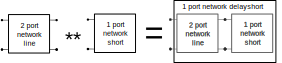
\includegraphics[width=0.7\linewidth]{figures/cascading.png}
	\caption{Cascading two 2-Port \texttt{Network}s in \skrf{} works with the \texttt{**} operator.}
	\label{fig:cascading}
\end{figure}

De-embedding can be accomplished by cascading the inverse of a network, as shown in Fig.~\ref{fig:deembedding}. This is implemented in \skrf{} through the property \texttt{Network.inv} property. To de-embed the short from \texttt{delayshort}:

\begin{lstlisting}[language=Python]
>>> short_2 = line.inv ** delayshort
>>> short_2 == short
True
\end{lstlisting}

\begin{figure}
	\centering
	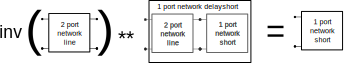
\includegraphics[width=0.9\linewidth]{figures/deembedding.png}
	\caption{Illustration of de-embedding using the inverse and cascade operators in \skrf{}.}
	\label{fig:deembedding}
\end{figure}

As shown in the previous example, Python comparison operators such as \texttt{==} also work with \texttt{Network} objects. 

\subsection{Statistical Analysis}
The \texttt{NetworkSet} class is useful for analysing multiple \texttt{.sNp} files initialized as \texttt{Network} objects or read from a directory. \texttt{NetworkSet}'s implement the same plotting routines as regular \texttt{Network}'s, which is convenient to plot a group of frequency responses. In addition, the \texttt{NetworkSet} class enables statistical analyses, such as calculating and plotting the uncertainty with the method \texttt{plot\_uncertainty\_bounds\_s\_db}. This is demonstrated in the following example, with the outputs shown in Fig.~\ref{fig:networkset}:

\begin{lstlisting}[language=Python]
from skrf.data import ro_1, ro_2, ro_3
ntwk_list = skrf.NetworkSet([ro_1, ro_2, ro_3])
ntwk_list.plot_s_db()
ntwk_list.plot_uncertainty_bounds_s_db(label='ro mean with uncertainty, S11')
\end{lstlisting}

\begin{figure}
	\centering
	\subfloat[]{
	    \includegraphics[width=0.45\textwidth]{figures/networkset_individual.pdf} 
	    \label{fig:networkset_individual}
	}
	\subfloat[]{
	    \includegraphics[width=0.45\textwidth]{figures/networkset_uncertainty.pdf} 
	    \label{fig:networkset_uncertainty}
	}
	\caption{Logarithmic magnitudes of $S_{11}$ of the \texttt{ro} example networks. (a) Individual frequency responses. (b) Calculated average and uncertainty bound ($3 \sigma$).}
	\label{fig:networkset}
\end{figure}

The standard deviations of data in a \texttt{NetworkSet} can be applied to a variety of attributes. The method \texttt{uncertainty\_ntwk\_triplet} can be utilized for gain output, similar to the previous example. For that case, the arguments \texttt{s\_mag} and \texttt{3} are used to specify that the uncertainty bounds should be for the magnitude of the scattering parameters within the range of 3 standard deviations. The \texttt{Network} objects generated by this function can be saved in various formats to be reused later:

\begin{lstlisting}[language=Python]
ntwk_mean, ntwk_lb, ntwk_ub = ntwk_list.uncertainty_ntwk_triplet('s_mag', 3)
\end{lstlisting}

\subsection{Interpolation and Concatenation}
A common need is to change the number of frequency points of a \texttt{Network}, for instance, but the previous operators and cascading functions require the networks to have matching frequencies:

\begin{lstlisting}[language=Python]
>>> from skrf.data import wr2p2_line1 as line1
# next line fails due to different frequencies
>>> line1 + line 
# next line works
>>> line.interpolate_from_f(line1.frequency) + line1  
\end{lstlisting}

A related application is the need to combine networks which cover different frequency ranges. Two \texttt{Network}s can be concatenated (stitched) using \texttt{stitch()}, which concatenates the \texttt{Network}s along their frequency axis. For example, to combine a WR-2.2 \texttt{Network} with a WR-1.5 \texttt{Network}:

\begin{lstlisting}[language=Python]
>>> from skrf.data import wr2p2_line, wr1p5_line
>>> big_line = skrf.stitch(wr2p2_line, wr1p5_line)
\end{lstlisting}

\subsection{Port Impedance Re-Normalization}
Scattering parameters are defined for a given reference impedance $Z_0$. It can be necessary to re-normalize these parameters to a different reference impedance. This example demonstrates how to use \skrf{} to re-normalize the  scattering parameters of a \texttt{Network} to different port impedances. Although trivial, this example creates a matched load in \SI{50}{\ohm} and then re-normalizes to a \SI{25}{\ohm} environment, producing a reflection coefficient of $1/3$. In case of complex reference impedances, \skrf{} supports both power-waves and pseudo-waves scattering parameter definitions \cite{williams2013}.

\begin{lstlisting}[language=Python]
>>> match_at_50 = skrf.wr10.match()
>>> match_at_50
1-Port Network: '',  75.0-110.0 GHz, 1001 pts, z0=[50.+0.j]
>>> match_at_50.s[0]  # S-parameter for the first frequency point
array([[0.+0.j]])
>>> match_at_50.renormalize(25)
>>> match_at_50
1-Port Network: '',  75.0-110.0 GHz, 1001 pts, z0=[25.+0.j]
>>> match_at_50.s[0]
array([[0.33333333+0.j]])
\end{lstlisting}

\section{Calibration}
It is possible with \skrf{} to calibrate a device under test (DUT), assuming that an acceptable set of standards have been measured and a corresponding set of ideal responses is known. This may be referred to as \textit{offline} calibration, because it is not occurring on-board the VNA itself. One benefit of this technique is that it provides maximal flexibility for non-conventional calibrations, and preserves all raw data. Self-calibration algorithms, such as Thru-Reflect-Line (TRL)\cite{engen1979}, do not require predefined ideal responses.

Several calibration routines are available in \skrf{}, for single port, two-ports or multi-ports networks. Traditional 12-terms \cite{marks1997} or 16-terms \cite{silvonen1993} error models are available, as well as 8-terms models \cite{speciale1977}, Short-Open-Load-Thru (SOLT) \cite{kruppa1971}, overdetermined one-port \cite{bauer1974}, Unknown-Thru \cite{ferrero1992}, Short-Delay-Delay-Load (SDDL) \cite{liu2006}, and some special algorithms developed by our contributors. In some cases, it may be necessary or desirable to use a one-port network analyser to determine the full set of scattering parameters of a two-port device. This technique is called one-port two-tier calibration \cite{ou2005} and is also implemented in \skrf{}. A complete list can be found on the \skrf{} website and only a single one-port is given as an example in this section.

\subsection{One-Port Example}
A calibration in \skrf{} is generated using the \texttt{Calibration} object. In general, \texttt{Calibration} objects require two arguments: a list of measured \texttt{Network}’s and a list of ideal \texttt{Network}’s. The following example assumes that a set of measured and ideal network standards are stored in separate directories named \texttt{ideals} and \texttt{measured}, for example a conventional short-open-load (SOL) calibration kit. These are used to create a one-port \texttt{Calibration} and to subsequently correct a measured DUT:

\begin{lstlisting}[language=Python]
from skrf.calibration import OnePort
# reads all Touchstone files located in the specified directory
my_ideals = skrf.load_all_touchstones_in_dir('ideals/')
my_measured = skrf.load_all_touchstones_in_dir('measured/')
# create a Calibration instance
cal = skrf.OnePort(\
    ideals = [my_ideals[k] for k in ['short','open','load']],
    measured = [my_measured[k] for k in ['short','open','load']],
)
# run calibration algorithm
cal.run()
# apply it to a DUT
dut = skrf.Network('my_dut.s1p')
dut_caled = cal.apply_cal(dut)
\end{lstlisting}

%\subsection{Two-Port Calibrations}
%Two-port calibrations are more involved than one-port. \skrf{} supports a few different two-port algorithms. The traditional SOLT algorithm uses the 12-term error model. This algorithm is straightforward, and similar to the \texttt{OnePort} example. The \texttt{EightTerm} calibration is based on the algorithm described in \cite{speciale1977}. It can be constructed from any number of standards, providing that some fundamental constraints are met. In short, you need three two-port standards; one must be transmissive, and one must provide a known impedance and be reflective. Note, that the word 8-term is used in the literature to describe a specific error model used by a variety of calibration algorithms, like TRL, LRM, etc. The \texttt{EightTerm} class, is an implementation of the algorithm cited above, which does not use any self-calibration.

\subsection{Multi-Line TRL Calibration}
\skrf{} can also be used for wideband Thru-Reflect-Line (TRL) calibration using multiple lines \cite{marks1991}. The necessary calibration standards in TRL calibration involve at least two transmission lines of different lengths and one or more reflective loads. Exact responses of the transmission lines and reflective loads does not need to be known and will be solved during the calibration. Ordinary SOLT or LRRM \cite{davidson1990} calibration usually moves the reference plane after the calibration to the SMA connector or probe tip used to contact the calibration standards. TRL calibration can be used to move the reference planes to the transmission lines on the substrate being measured if every measured standard includes a similar launch to the transmission lines. This makes TRL calibration very useful when accurate short, open, load and thru standards cannot be manufactured, or when the measurement reference plane needs to be on the substrate being measured. 

\section{Time-Domain and Gating}
Time-gating is a processing technique which is commonly used to pinpoint a response of interest in the presence of multiple reflections in order to isolate their effects \cite{cronson1973, bennett1978}. This is commonly done on-board a VNA. However, if instead the time-gating occurs offline on a computer, the user can keep the raw measurements separate from the processed results. This is important so that the processing algorithm can be altered in the future without remeasuring the data. 

\begin{figure}
	\centering
	\subfloat[]{\includegraphics[width=0.45\textwidth]{figures/gating_timedomain.pdf} \label{fig:gating_timedomain}}
	\subfloat[]{\includegraphics[width=0.45\textwidth]{figures/gating_freqdomain.pdf} \label{fig:gating_freqdomain}}
	\caption{Comparison of the original network response $S_{11}$ with its gated version. (a) In the time-domain. (b) In the frequency-domain.}
	\label{figs:gating}
\end{figure}

In the following example, the time-gating functions of \skrf{} are used to filter out the effects of an undesired reflection. This can be done by using the method \texttt{Network.time\_gate}, and provide it an appropriate centre and span (in nanoseconds):

\begin{lstlisting}[language=Python]
probe_s11 = skrf.Network('./probe.s2p').s11
probe_s11.name = 'Probe'
probe_s11_gated = probe_s11.time_gate(center=0, span=0.2)
probe_s11_gated.name = 'Gated probe'
# time-domain plot:
s11.plot_s_db_time()
s11_gated.plot_s_db_time()
# frequency-domain plot:
s11.plot_s_db()
s11_gated.plot_s_db()
\end{lstlisting}

To see the effects of the gate, both the original and gated response are compared. As shown in Fig.~\ref{figs:gating}, the original response shows an interference pattern in the frequency-domain due to this undesirable reflection at \SI{0.2}{\nano\second}. After gating, the response is cleaned.


\section{Circuit Building}
\skrf{} enables the building of a circuit with arbitrary topology, consisting of an arbitrary number of $N$-port \texttt{Network}'s connected together. Similar to an electronic circuit simulator, the circuit must have one or more ports connected to the circuit. With the \texttt{Circuit} object, the combined responses of the $M$-port network can be calculated (and thus its network parameters: $S$, $Z$, etc.), where $M$ is the number of ports defined. Moreover, the \texttt{Circuit} object also allows calculating the scattering matrix $S$ of the entire circuit, that is the "internal" scattering matrices for the various intersections in the circuit. The calculation algorithm is based on \cite{hallbjorner2003}.

\begin{figure}
	\centering
	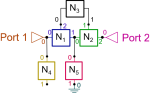
\includegraphics[width=0.5\linewidth]{figures/circuit.png}
	\caption{ Example of a \texttt{Circuit} made of various kinds of $N$-port \texttt{Network}'s.}
	\label{fig:circuit}
\end{figure}

Fig.~\ref{fig:circuit} illustrates a network with 2 ports, \texttt{Network} elements $N_i$ and intersections. In order to define such a circuit, the connection list needs to be defined, which describes how the networks are connected:

\begin{lstlisting}[language=Python]
connections = [
[(network1, network1_port_nb), (network2, network2_port_nb), (network2, network2_port_nb), ...], 
...
]
\end{lstlisting}

The connection list to construct the \texttt{Circuit} illustrated in Fig.~\ref{fig:circuit} could be:

\begin{lstlisting}[language=Python]
>>> connections = [
[(port1, 0), (network1, 0), (network4, 0)],
[(network1, 1), (network2, 0), (network5, 0)],
[(network1, 2), (network3, 0)],
[(network2, 1), (network3, 1)],
[(network2, 2), (port2, 0)],
[(network5, 1), (ground1, 0)]
]
\end{lstlisting}

In this example, the \texttt{Circuit} elements \texttt{port1}, \texttt{port2}, \texttt{ground1} and all the \texttt{network1} to \texttt{network5} are assumed to be \skrf{} \texttt{Network} objects with the same \texttt{Frequency} attribute. The individual networks can have different (real) reference impedances and mismatches are taken into account. Note that port 1 of \texttt{network4} is left open, so is not described in the connection list. Once the connection list is defined, the \texttt{Circuit} is built with:

\begin{lstlisting}[language=Python]
resulting_circuit = skrf.Circuit(connections)
\end{lstlisting}

The resulting 2-ports \texttt{Network} is obtained with \texttt{Circuit.network}:
\begin{lstlisting}[language=Python]
resulting_network = resulting_circuit.network
\end{lstlisting}

%Note that it is also possible to manually create a \texttt{Circuit} from multiple \texttt{Network} objects using the connection methods of \skrf{}. Although the \texttt{Circuit} approach to build network connection may appear to be more verbose than the "classic" way for building a circuit, as the circuit complexity increases, in particular when components are connected in parallel, the \texttt{Circuit} approach is interesting as it increases the readability of the code. Moreover, a \texttt{Circuit}'s topology can be plotted using its \texttt{plot\_graph} method, which is useful to rapidly control if the circuit is built as expected.


\section{Vector Fitting}
Microwave circuit design requires simulations in the time or frequency-domain with accurate models of all involved circuit elements. For passive structures, electromagnetic field simulations or measurements can provide accurate network models in the form of sampled frequency responses, but these cannot directly be used in circuit simulators such as SPICE. To translate the sampled frequency responses of a $N$-port network into a model for circuit simulations, \skrf{} provides an implementation of the well-known vector fitting algorithm to fit the samples in the frequency-domain \cite{vectfit}. The rational basis functions used for the fit enable the subsequent generation of linear equivalent circuits based on resistors, capacitors, inductors, and controlled current and voltage sources to be used in most types of circuit simulators \cite{vectfit_spice}. 

To summarize the vector fitting approach, the vector $\mathbf{H}(\mathrm{s})$ represents the stack of fitting functions for the $N \cdot N$ individual network responses defined in the Laplace domain with $\mathrm{s} = \sigma + \mathrm{j} \omega$:

\begin{equation}
\mathbf{H}(\mathrm{s}) = \mathbf{d} + \mathrm{s} \, \mathbf{e} + \sum _{k=1} ^{K} \frac{\mathbf{z}_k}{\mathrm{s} - p_k}.
\label{eq:vectfit_function}
\end{equation}

In (\ref{eq:vectfit_function}), $\mathbf{H}(\mathrm{s})$ includes a series of $K$ rational fractions with a common set of poles $p_k$ for all the responses of the network, but with individual zero vectors $\mathbf{z}_{k}$, as well as individual constant and proportional vectors $\mathbf{d}$ and $\mathbf{e}$, respectively.

For example, the scattering parameters of a 2-port can be subjected to vector fitting with $K$ poles. The objective is therefore to match the original network samples at all sampling frequencies $\omega_m \in [\omega_1, \omega_2, \cdots, \omega_M]$:

\begin{equation}
\begin{pmatrix}
S_{11} (\omega_m) \\
S_{12} (\omega_m) \\
S_{21} (\omega_m) \\
S_{22} (\omega_m)
\end{pmatrix} 
\overset{!}{=}
\begin{pmatrix}
d_{11} + \mathrm{j} \omega_m e_{11} + \sum _{k=1} ^{K} \frac{z_{k,11}}{\mathrm{j} \omega_m - p_k} \\
d_{12} + \mathrm{j} \omega_m e_{12} + \sum _{k=1} ^{K} \frac{z_{k,12}}{\mathrm{j} \omega_m - p_k} \\
d_{21} + \mathrm{j} \omega_m e_{21} + \sum _{k=1} ^{K} \frac{z_{k,21}}{\mathrm{j} \omega_m - p_k} \\
d_{22} + \mathrm{j} \omega_m e_{22} + \sum _{k=1} ^{K} \frac{z_{k,22}}{\mathrm{j} \omega_m - p_k}
\end{pmatrix} .
\end{equation}

The fitting process involves running an iterative least-squares algorithm \cite{vectfit}, which is implemented in \skrf{} including the speed improvements proposed in \cite{vectfit_improved} and \cite{vectfit_fast}.

In \skrf{}, the class \texttt{VectorFitting} is instanced with the \texttt{Network} to be fitted. A subsequent call of the \texttt{vector\_fit} routine starts the fitting process with the number of real and complex-conjugate poles defined in the function arguments. Once the fitting is finished, the function \texttt{write\_spice\_subcircuit\_s} can be called to generate a SPICE subcircuit file based on the fitted poles $\mathbf{p}$, zeros $\mathbf{z}$, constants $\mathbf{d}$, and proportional coefficients $\mathbf{e}$ of the scattering parameter responses:

\begin{lstlisting}[language=Python]
nw = skrf.Network('example.s4p')
vf = skrf.VectorFitting(nw)
vf.vector_fit(n_poles_real=2, n_poles_cmplx=32)
vf.write_spice_subcircuit_s('example.sp')
\end{lstlisting}

\begin{figure}
\centering
\subfloat[]{\includegraphics[width=0.45\textwidth]{./figures/vectfit_magnitude.pdf} \label{fig:vectfit_magnitude}}
\hfill
\subfloat[]{\includegraphics[width=0.45\textwidth]{./figures/vectfit_error.pdf} \label{fig:vectfit_error}}
\\
\subfloat[]{\includegraphics[width=0.7\textwidth]{./figures/vectfit_spice.pdf} \label{fig:vectfit_spice}}
\caption{Selected scattering parameter responses of a vector fitted noisy 4-port example network. (a) Magnitudes in linear scale with markers for the samples and solid lines for the fit. (b) Absolute error magnitudes of the respective fits: absolute error $ = |S_{\mathrm{fit},i,1} - S_{\mathrm{sample},i,1}|$. (c) Simulation of the scattering parameters with \textit{ngspice} using the exported SPICE subcircuit.}
\label{figs:vectfit}
\end{figure}

In Fig. \ref{fig:vectfit_magnitude} and \ref{fig:vectfit_error}, four of the 16 vector fitted scattering parameter responses of the example network are plotted and compared to the original network samples, showing an absolute error of less than $0.01$. SPICE simulations using the exported subcircuit file in \textit{ngspice} \cite{ngspice_website} achieve a similar accuracy. The simulated scattering parameter obtained from an AC simulation are shown in Fig. \ref{fig:vectfit_spice}.

The quality of the fit strongly depends on the choice of real and complex-conjugate starting poles, which should suit the number of resonances in the responses. Measurement noise in the sampled responses, as included in this 4-port example, further contributes to the deviation of the fit with the smooth basis functions used by the vector fitting method. The translation of the fitting parameters into the SPICE equivalent subcircuit is straightforward, and the accuracy is only limited by rounding errors. However, the accuracy of the simulation results also depends on the tolerance settings of the simulator.

\section{Conclusion}
\skrf{} is an open-source Python package produced for RF/Microwave engineering. The package provides a modern, object-oriented library for RF network analysis, circuit building and calibration. Below is a current non-exhaustive feature list of \skrf{} (as of version 0.18).

\begin{itemize}
	\item	Microwave network operations
	\begin{itemize}
	\item	Read/Write touchstone (.sNp) files
	\item	S/Z/Y/ABCD/T - parameter conversions
	\item	Arithmetic operations on scattering parameters
	\item   Mixed mode and single ended port conversion
	\item	Cascade/De-embed Networks
	\item	Frequency and port slicing and concatenation.
	\item   Assembly of multiple-port networks
	\item   Vector fitting (S, Z, Y parameters) and export of equivalent SPICE subcircuits (based on S parameters only)
	\end{itemize}
\item	Sets of Networks:
	\begin{itemize}
		\item Statistical properties of a set of Network
		\item Interpolation between a set of Network (frequency or parametric)
		\item Methods to sort and visualize set behaviour
	\end{itemize}
\item	Plotting abilities:
	\begin{itemize}
		\item Rectangular plots (dB, magnitude, phase, group delay)
		\item Smith chart
		\item Automated uncertainty bounds
	\end{itemize}
\item	Calibration Routines:
	\begin{itemize}
		\item One-Port: SOL, Least Squares, SDDL
		\item Two-Port: TRL, Multiline TRL, SOLT, Unknown Thru, 8/16-Term
		\item Partial : Enhanced Response, One-Port Two-Path
	\end{itemize}
\item	Virtual Instruments (completeness varies by model)
	\begin{itemize}
		\item VNAs: PNA, PNAX, ZVA, HP8510, HP8720
		\item SA: HP8500
		\item Others: ESP300
	\end{itemize}
\item	Transmission Line Physics:
	\begin{itemize}
		\item Distributed Circuit, Coaxial/Coplanar/Rectangular/Circular Waveguides, Free-space, 
		\item Transmission line voltage, current, power and losses calculations
		\item Complex characteristic impedance support
	\end{itemize}

\end{itemize}

In addition to these rich features, there are also GUIs for time gating and sNp file viewing, with source code available at \href{https://github.com/scikit-rf/dash-apps}{\UrlFont{https://github.com/\skrf{}/dash-apps}} and functional demos hosted by Plotly at \url{https://dash-gallery.plotly.host/Portal/}. 

\section{Contributing}
\skrf{} is a free and open-source project. For those seeking help or reporting bugs, there is a public mailing list and GitHub issues tracker which can be found on the \skrf{} website (\href{https://skrf.org}{\UrlFont{https://\skrf{}.org}}). If you would to participate in development, first join GitHub (\url{https://github.com}) and then take a look at the \skrf{} development pages. For companies or individuals who need private support and development services, feel free to contact 810 Labs LLC (\url{http://810lab.com/}).

%%%%%%%% ACKNOWLEDGMENT
\section*{Acknowledgment}
\skrf{} would not be possible without the feedback, bug fixes, and new features contributed by its user community. Visit \href{https://github.com/scikit-rf/scikit-rf/graphs/contributors}{\UrlFont{https://github.com/\skrf{}/\skrf{}/graphs/contributors}} to see a full list of contributors.

%%%%%%%% REFERENCES
\bibliographystyle{ieeetr}
\bibliography{IEEEabrv, biblio}

\end{document}
